\documentclass[fontscale=0.33,landscape,paperwidth=48in,paperheight=36in]{baposter}  % fontscale=0.285, dvipdfm

\usepackage{setspace}
\usepackage{multicol}
\usepackage{multirow}

\usepackage{tikz}
%\usepackage{pgfbaselayers}
%\pgfdeclarelayer{background}
%\pgfdeclarelayer{foreground}
%\pgfsetlayers{background,main,foreground}

%%% Color Definitions %%%%%%%%%%%%%%%%%%%%%%%%%%%%%%%%%%%%%%%%%%%%%%%%%%%%%%%%%

\selectcolormodel{cmyk}

\definecolor{bordercol}{RGB}{0,0,0}
%\definecolor{headercolone}{RGB}{6,130,22}
\definecolor{headercol}{cmyk}{1,0.64,0,0.6}
%\definecolor{headercolone}{cmyk}{1,0.64,0,0.6}
%\definecolor{headercoltwo}{cmyk}{0.44,0,0.15,0.17}
%\definecolor{headercolone}{cmyk}{0.3,0,0.15,0.17}
%\definecolor{headercoltwo}{cmyk}{0.3,0,0.15,0.17}
\definecolor{iumint}{cmyk}{0.40,0,0.23,0}
\definecolor{iumidnight}{cmyk}{0.71,0.30,0.13,0.41}
%\definecolor{boxcolor}{RGB}{176,208,223}
%\definecolor{boxcolor}{cmyk}{0.3,0.08,0.08,0.1}
\definecolor{boxcolor}{cmyk}{0.2,0.03,0.03,0.1}
\definecolor{headerfontcol}{RGB}{255,255,255}
\newcommand{\hilitetwo}[1]{{\addfontfeature{Color=99333399}#1}}
\newcommand{\hiliteone}[1]{{\addfontfeature{Color=06821699}#1}}
\newcommand{\hilitegrey}[1]{{\addfontfeature{Color=77777799}#1}}
\newcommand{\hilitelightgrey}[1]{{\addfontfeature{Color=CCCCCC99}#1}}
\newcommand{\hiliteblue}[1]{{\addfontfeature{Color=44697DFF}#1}}

%%% Utility functions %%%%%%%%%%%%%%%%%%%%%%%%%%%%%%%%%%%%%%%%%%%%%%%%%%%%%%%%%%

%%% Save space in lists. Use this after the opening of the list %%%%%%%%%%%%%%%%
\newcommand{\compresslist}{
        \setlength{\itemsep}{1pt}
        \setlength{\parskip}{0pt}
        \setlength{\parsep}{0pt}
}

\usepackage{polyglossia}
\setdefaultlanguage[variant=australian]{english}

\usepackage{expex}

\usepackage{fontspec}
\defaultfontfeatures{PunctuationSpace=2,Scale=MatchLowercase,Mapping=tex-text}
\newfontfeature{IPA}{+mgrk}
%\setromanfont[IPA]{FreeSerif}
%\setromanfont[IPA,Scale=0.8]{CMU Serif}
%\setromanfont[IPA]{Liberation Serif}
\setromanfont[IPA]{Linux Libertine O}
%\setromanfont[IPA]{Nimbus Roman No9 L}
\setmonofont[IPA]{DejaVu Sans Mono}
\usepackage[small,bf]{caption}
\newfontfamily\qipa[IPA,Scale=MatchLowercase]{FreeSerif}
\newfontfamily\qgmk[IPA,Scale=0.8]{CMU Serif}
\newfontfamily\litamono[IPA,Scale=0.5]{DejaVu Sans Mono}
\newfontfamily\ortamono[IPA,Scale=0.625]{DejaVu Sans Mono}

\newcommand{\tilda}{{\qipa ∼}}

\newcommand{\tags}[1]{\hiliteone{#1}}
\newcommand{\tag}[1]{{\ortamono \hilitegrey{<}\hiliteblue{#1}\hilitegrey{>}}}
\newcommand{\archiphon}[1]{\hilitegrey{\{}\hiliteone{#1}\hilitegrey{\}}}

%\newfontfamily\htwo[IPA,Scale=1.2]{FreeSans}}
%\newfontfamily\htwofont[IPA,Scale=1]{CMU Sans Serif}
%\newfontfamily\htwofont[IPA,Scale=1,Color=333344FF]{CMU Sans Serif}
\newfontfamily\htwofont[IPA,Scale=1,Color=111111FF]{CMU Sans Serif}
%\newfontfamily\titlefont[IPA,Scale=0.52]{CMU Serif}
%\newfontfamily\titlefont[IPA,Scale=0.7]{CMU Serif}
%\newfontfamily\titlefont[IPA,Scale=0.7]{CMU Sans Serif Demi Condensed}
\newfontfamily\titlefont[
	%SmallCapsFont={Andika},
	%SmallCapsFont={Alegreya Sans SC},
	SmallCapsFont={Andada SC},
	%SmallCapsFont={Carrois Gothic SC},
	SmallCapsFeatures={Letters=SmallCaps},
	Scale=0.8,
]{Andada SC}
%\newfontfamily\titlefont[IPA,Scale=0.7]{Nimbus Sans L}
%\newfontfamily\titlefont[IPA,Scale=0.55]{DejaVu Serif}

%\newcommand{\htwo}[1]{::: {\htwofont #1} :::}%\hrule} %\hline\\}
%\newcommand{\htwo}[1]{{\htwofont \textbf{:::#1:::}}}%\hrule} %\hline\\}
\newcommand{\htwo}[1]{{\htwofont \textbf{\dotfill{}#1\dotfill{}}}}


\usepackage{graphicx}  % [dvipdfm]

%\definecolor{MyGray}{rgb}{0.96,0.97,0.98}
%\newenvironment{codebox}{%
%   \begin{lrbox}{\@tempboxa}\begin{minipage}{\columnwidth}}{\end{minipage}\end{lrbox}%
%   \colorbox{MyGray}{\usebox{\@tempboxa}}
%}
%\newcommand{\codeex}[1]{\begin{codebox}#1\end{codebox}}

%\definecolor{grey}{rgb}{0.96,0.97,0.98}
\definecolor{grey}{rgb}{0.91,0.91,0.91}
\newcommand{\codeex}[1]{
   \fbox{\colorbox{grey}{
         \begin{minipage}[t]{0.91\textwidth}{\litamono
				\begin{spacing}{0.4}
	            #1
				\vspace{-1em}\end{spacing}
         }\end{minipage}
      }
   }
}
\newcommand{\outputex}[1]{
   \fbox{\colorbox{iumidnight}{
         \begin{minipage}[t]{0.91\textwidth}{\ortamono
				\begin{spacing}{0.2}\vspace{-0.8em}
	            \hilitelightgrey{#1}
				\vspace{-2.5em}\end{spacing}
         }\end{minipage}
      }
   }
}



\newcommand{\blank}[1]{\underline{\hspace{#1}}}

\usepackage{natbib}

\usepackage[colorlinks=true,citecolor=black,linkcolor=black,urlcolor=black]{hyperref}

\usepackage{subfigure}
\usepackage{booktabs}

%%\bibpunct{(}{)}{;}{A}{,}{,}
%\bibdata{paper}

\newcommand{\citemultileft}[1]{(\citeauthor{#1}, \citeyear{#1}}
\newcommand{\citemultimid}[1]{\citeauthor{#1}, \citeyear{#1}}
\newcommand{\citemultiright}[1]{\citeauthor{#1}, \citeyear{#1})}
\newcommand{\citetwoyears}[2]{\citeauthor{#1} (\citeyear{#1} and \citeyear{#2})}

% for glosses
\newcommand{\eng}[1]{`{\em #1}'}
%dammit, sc doesn't seem to be working
\newcommand{\gmk}[1]{{\qgmk \textsc{#1}}}


\usepackage{enumitem}
\setlist{nolistsep,leftmargin=*}
\newenvironment{itemise}[1]{
        \begin{itemize}\setlength{\leftmargin}{-4em}\setlength{\itemsep}{-0.2em}
        \vspace{-0.5em}
        #1
}{
        \end{itemize}
        \vspace{-2pt}
}

%\newcommand{\h2}[1]{{\big



\begin{document}
	% To get it to be the same size consistently on all machines..
	\special{papersize=48in,36in}
	\setlength{\pdfpageheight}{\paperheight}
	\setlength{\pdfpagewidth}{\paperwidth}

	%%% Setting Background Image %%%
	%\background{}

	\begin{poster}{
		grid=false,
		%eyecatcher=false,
		borderColor=bordercol,
		headerColorOne=iumidnight,
		headerColorTwo=iumidnight,
		%headerColorOne=blue,
		headerFontColor=white,
		% Only simple background color used, no shading, so boxColorTwo isn't necessary
		boxColorOne=boxcolor,
		headershape=roundedright,
		headerborder=open,
		headerheight=0.1\textheight,
		%headershape=roundedright,
		%headershade=plain,
		%headerfont=\Large\textsf, %Sans Serif
		%headerfont=\Large\sf\bf,
		textborder=rectangle,
		%background=plain,
		%background=user,
		background=none,
		headerborder=open,
		boxshade=plain,
		textborder=roundedleft,
		columns=4,
	}{ %Eye Catcher, empty if option eyecatcher=false - unused
		
\includegraphics[height=6.5em]{uitlogo}
		\hspace{2.5cm}\begin{minipage}[t]{7em}
			\vspace{-2cm}
			\noindent
\includegraphics[height=4.2em]{DCU_logo_2col}\\
			\vspace{-0.5ex}\hspace{0.105cm}
\includegraphics[height=2.15em]{DCU_2010_Name_Mark_289}
		\end{minipage}

	}{ %Title (centered top)
		{%\vspace{0pt}\hspace{1cm} \
			{\titlefont \scshape{Finite-State Morphologies \& Text Corpora\\\vspace{0.2em}\scalebox{0.8}{as Resources for Improving Morphological Descriptions}}}}
	}{ %Authors (centered top, below title)
		\vspace{-0.6em}
		\begin{center}
			\begin{minipage}[t]{9em}
				\begin{spacing}{0.4}
				{Francis M.\ Tyers}\\
				{\footnotesize UiT Norgga Árktalaš Universitehta \\\texttt{francis.tyers@uit.no}}
				\end{spacing}
			\end{minipage}
			\begin{minipage}[t]{9.5em}
				\begin{spacing}{0.4}
					{Tommi Pirinen\vphantom{y}}\\
					{\footnotesize Ollscoil Chathair Bhaile Átha Cliath\vphantom{y}\\\texttt{tommi.pirinen@computing.dcu.ie}}
				\end{spacing}
			\end{minipage}
			\begin{minipage}[t]{12em}
				\begin{spacing}{0.4}
					{Jonathan North Washington}\\
					{\footnotesize Indiana University\\\texttt{jonwashi@indiana.edu}}
				\end{spacing}
			\end{minipage}
		\end{center}
	}{ %More eye catchers, on the right side
		
\includegraphics[height=6.25em]{iu_tab-crop}
		\hspace{2.5cm}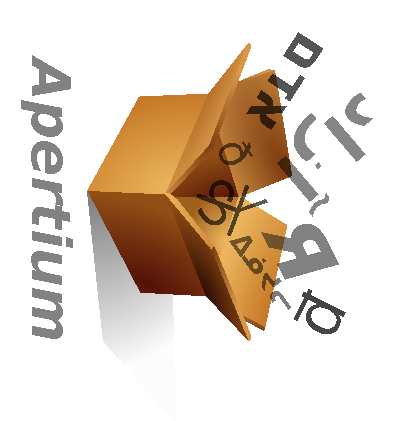
\includegraphics[angle=90,height=6.8em]{apertium5b}%\hspace{-2em}
	}

	\headerbox{Morphological Descriptions}{name=morphdesc,column=0,row=0}{
		\htwo{What are they?}
		\begin{itemize}
			\item core part of grammatical descriptions
			\item found in reference grammars and textbooks
		\end{itemize}

		\htwo{What they describe} %Describe a language's
		\begin{itemize}
			\item \textbf{morphotactics} — the morphemes of a language and how they can be combined
			\item \textbf{morphophonology} — the alternations between the various phonological and orthographical forms of each morpheme% in a language
		\end{itemize}
		
		\htwo{Reasons for being \hilitetwo{incomplete}}
		\begin{itemize}
			\item restrictions of the medium (e.g., number of pages)
			\item limitations of introspection, working with native speakers
			\item \textbf{lack of automatic testing}
		\end{itemize}
	}
	
	\headerbox{Morphological transducers}{name=morphtrans,below=morphdesc}{
		\htwo{Morphological transducers}
		\begin{itemize}
			\item Efficient (in speed \& size) models of a language's morphology
			\item Take a surface form, and produce valid lexical form(s)
			\item Take a lexical form, and produce valid surface form(s)\vspace{-0.1ex}\\
		%\end{itemize}
		\scalebox{0.98}{
			алдым \hilitetwo{↔} \texttt{ал\tag{v}\tag{tv}\tag{ifi}\tag{p1}\tag{sg}}, \texttt{алд\tag{n}\tag{px1sg}\tag{nom}}
		}
		\end{itemize}

		\htwo{Turkic-language transducers we've made}
		\begin{itemize}
			%\item Turkish (\hiliteone{Çöltekin, 2010 \& 2014}; \hilitetwo{Oflazer, 1994})
			%\item Crimean Tatar (\hilitetwo{Altıntaş, 2001})
			%\item Turkmen (\hilitetwo{Tantuğ et al., 2006})
			%\item Kazakh (\hilitetwo{Бекманова \& Махимов, 2013})
			%\vspace{1pt}\hfill{} \hiliteone{GPL (=free and open)}!
			%\item our Kyrgyz, Kazakh, Tatar, Kumyk:\ all \hiliteone{GPL (=free and open)}!
			\item Kyrgyz (Washington et al., 2012)
			\item Tatar \& Bashkort (Tyers et al., 2012)
			\item Kazakh (Salimzyanov et al., 2013)
			\item Kumyk (Washington et al., 2014)
			\item ongoing work on Sakha, Tuvan, Khakas, and more!
		\end{itemize}

		\htwo{Framework:\ HFST}
		\begin{itemize}
			\item Reimplements Xerox FST formalisms ({\tt lexc} \& {\tt twol})
			\item Also provides a wrapper around popular free/open-source FST toolkits: SFST, OpenFST, and Foma
		\end{itemize}
		\htwo{Approach}
		\begin{itemize}
			\item morphotactics implemented in \texttt{lexc}
			\item morphophonology implemented in \texttt{twol} (SPE-style rules)
			\item compiled separately; compose-intersected to single transducer\vspace{-0.1ex}\\
			алдым\hfill{}\hilitetwo{↔}\hfill{}\texttt{ал\hilitegrey{>}\archiphon{D}\archiphon{I}\hilitegrey{>}м}\hfill{}\hilitetwo{↔}\hfill{}\texttt{ал\tag{v}\tag{tv}\tag{ifi}\tag{p1}\tag{sg}}\vspace{-0.1ex}\\
			алдым\hfill{}\hilitetwo{↔}\hfill{}\texttt{алд\hilitegrey{>}\archiphon{I}м}\hfill{}\hilitetwo{↔}\hfill{}\texttt{алд\tag{n}\tag{px1sg}\tag{nom}}
		\end{itemize}

	}

	\headerbox{Example: Categorisation}{name=adjectives,column=3}{
		\htwo{Unrestricted 0-derivation}
		\begin{itemize}
			\item Common overgeneralisation of adjective morphology:
			\begin{itemize}
				\item all adjectives may act like nouns (i.e.\ take noun morphology)
				\item all adjectives may be used as is as adverbs
			\end{itemize}
			\item Commonly reported in Turkic language grammars
		\end{itemize}
		Somfai Kara (2002, pp. 28-29):\ 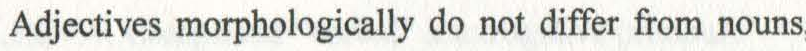
\includegraphics[width=0.53\textwidth]{img/kara28}\\
		\-\hfill{}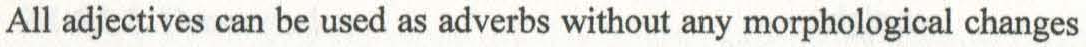
\includegraphics[width=0.8\textwidth]{img/kara29}

		\htwo{Attested system}
			\begin{itemize}
				\item Some adjectives may not be substantivised
				\item Some adjectives may not be used adverbially
				\item Some adjectives do not have comparative forms
				\item …a range of “adjective classes” in most Turkic languages
			\end{itemize}
		\htwo{Implementation}
			\begin{itemize}
				\item if properly categorised, only correct forms are analysed and generated
			\end{itemize}
				
			\scalebox{0.83}{
				\begin{tabular}{lllll}
					\toprule
					\textbf{Type} & \textbf{Gloss} & {\small \texttt{\tag{adj}(\tag{comp})}} & {\small \texttt{\tag{adj}(\tag{comp})\tag{subst}}} & {\small \texttt{\tag{adj}(\tag{comp})\tag{advl}}} \\
					\midrule
					\textbf{A1} & \eng{good} & {\qipa яхшы (яхшырак)} & {\qipa яхшы (яхшырак)} & {\qipa яхшы (яхшырак)} \\
					\textbf{A2} & \eng{old} & {\qipa иске (искерәк)} & {\qipa иске (искерәк)} & {\qipa — (—)} \\
					\textbf{A3} & \eng{dead} & {\qipa үле (—)} & {\qipa үле (—)} & {\qipa — (—)} \\
					\textbf{A4} & \eng{basic} & {\qipa төп (—)} & {\qipa — (—)} & {\qipa — (—)} \\
					\bottomrule
				\end{tabular}
			}\\
			This phenomenon is of particular interest because native-speaker intuitions on the morphological limitations of a given adjective can often be more restrictive than the range of possible uses found in a large text corpus.
	}

		\headerbox{Example:\ Tuvan velar elision}{name=tuvanvelars,column=1,span=2}{
			\begin{multicols}{2}
				\htwo{Previous descriptions}

					\begin{itemize}
						\item Anderson and Harrison (1999, pp.\ 9, 22-23)
					\end{itemize}
					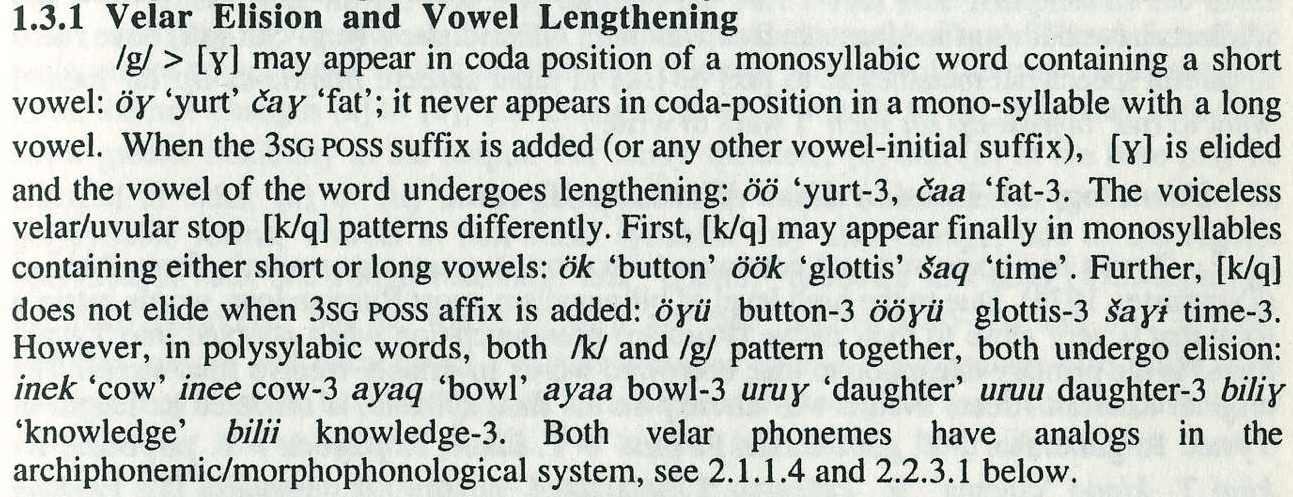
\includegraphics[width=0.49\textwidth]{img/andersonharrison9}\\
					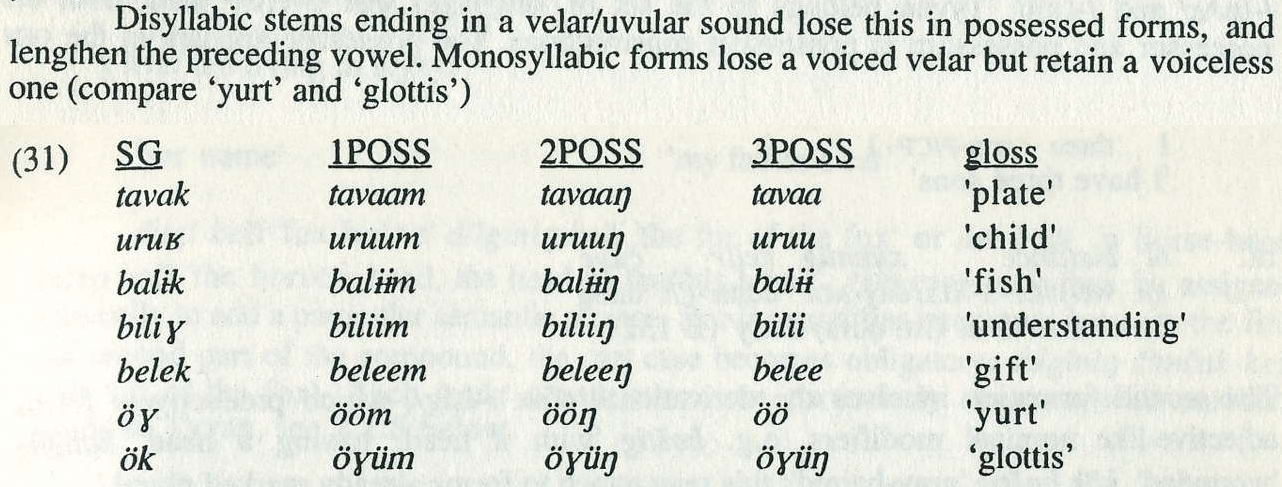
\includegraphics[width=0.49\textwidth]{img/andersonharrison22-23}
					\begin{itemize}
						\item Исхаков, Ф.Г.; Пальмбах (1961, pp.\ 117-118)
					\end{itemize}
					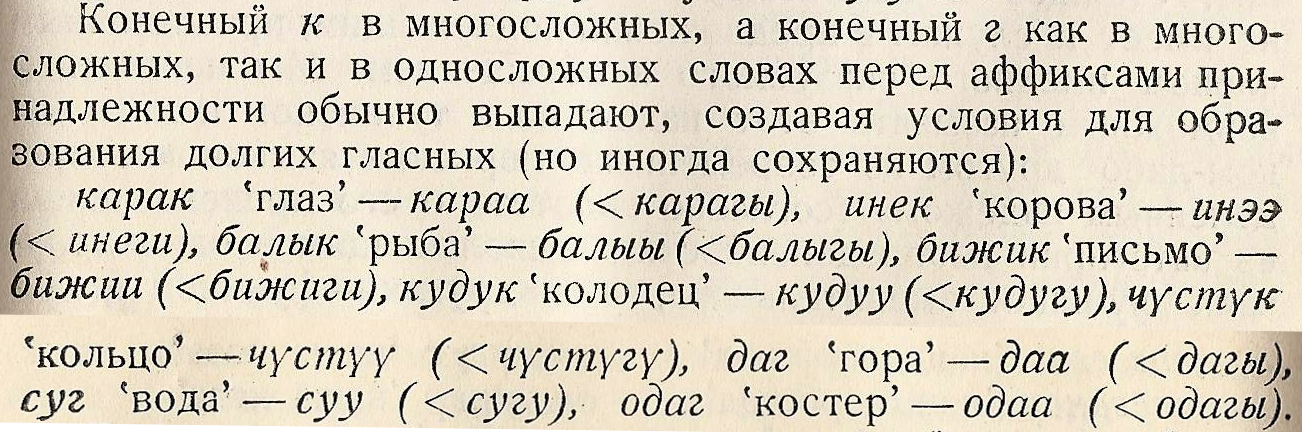
\includegraphics[width=0.49\textwidth]{img/isxakovpalmbax117}

				\htwo{More complete characterisation}
				\begin{itemize}
					\item /k/ ‹к› elides at the end of >1-σ stems intervocalically\\
						инэк+I → инээ, өк+I → өгү
					\item /g/ ‹г› elides at the end of any stem intervocalically\\
						өг+I → өө 
					\item /ŋ/ ‹ң› elides at the end of \textbf{some} stems intervocalically.\\
						\textbf{соң+I → соо}, чаң+I → чаңы, түң+I → түңү
				\end{itemize}

				\htwo{Correct forms in the grammars}

				But not part of the morphophonological description.\\
				(A. \& H., p.\ 35)\hfill{}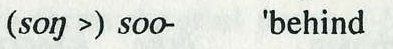
\includegraphics[width=0.2\textwidth]{img/andersonharrison35}\\
				(И.\ \& П., p.\ 447)\hfill{}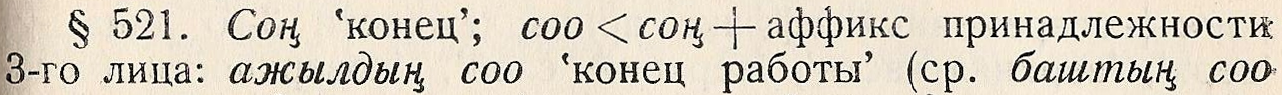
\includegraphics[width=0.35\textwidth]{img/isxakovpalmbax447}


			\columnbreak{}
				\htwo{Uanalysed forms before implementation}
					\begin{itemize}
						\item \hilitetwo{инээ}, \hiliteone{өгү}, \hilitetwo{өө}, \hilitetwo{соо}, \hiliteone{чаңы}
					\end{itemize}\vspace{-0.3ex}
					\begin{minipage}[t]{0.5\textwidth}
					\outputex{
						\begin{multicols}{4}
							1590 соонда\vphantom{ү}\\
							610 те\vphantom{ү}\\
							153 өөнүң\vphantom{ү}\\
							48 соондан\vphantom{ү}\\
							46 өөм\vphantom{ү}\\
							20 соон\vphantom{ү}\\
							18 өө\vphantom{ү}\\
							17 өөнге\vphantom{ү}\\
							9 соондагы\vphantom{ү}\\
							8 өөн\vphantom{ү}\columnbreak\\
							6 инээниң\vphantom{ү}\\
							6 соонче\vphantom{ү}\\
							6 соонга\vphantom{ү}\\
							3 инээм\vphantom{ү}\\
							3 өөнден\vphantom{ү}\\
							3 өөнде\vphantom{ү}\\
							3 өөмнүң\vphantom{ү}\\
							2 инээн\vphantom{ү}\\
							2 инээ\vphantom{ү}\\
							2 өөнче\vphantom{ү}\columnbreak\\
							2 өөңерге\vphantom{ү}\\
							2 өөңер\vphantom{ү}\\
							2 өөмнү\vphantom{ү}\\
							2 өөвүстен\vphantom{ү}\\
							2 өөвүске\vphantom{ү}\\
							2 өөвүс\vphantom{ү}\\
							1 инээңни\vphantom{ү}\\
							1 инээмниң\vphantom{ү}\\
							1 Инээм\vphantom{ү}\\
							1 инээвистиң\vphantom{ү}\\
							1 өөңнүң\vphantom{ү}\\
							1 өөң\vphantom{ү}\\
							1 өөвүсче\vphantom{ү}\\
							1 өөвүстүң\vphantom{ү}\\
							1 өөвүстү\vphantom{ү}\\
							1 өөвүсте
						\end{multicols}}
					\end{minipage}

				\htwo{Initial implementation}
					\begin{minipage}[t]{0.5\textwidth}
					\codeex{"Intervocalic voiced velar deletion"\\
г:0 <=> :Vow/:0* \_ [ \%>: :Vow ]/:0* ;\\
\-~\\
"Intervocalic voiceless velar deletion"\\
к:0 <=> :Vow/:0* \_ [ \%>: :Vow ]/:0* ;\\
\-~~~~except\\
\-~~~~~~~~[ .\#.\ | \%- ] [ ( :Cns* ) ( :Vow* ) :Vow ]/:0 \_ [ \%>:\ :Vow ]/:0* ; %[ :0 - \%>:\ ]* ;
					}
					\end{minipage}

				\htwo{Unanalysed forms after initial implementation}
					%(has forms of соң in it)
					\begin{itemize}
						\item \hiliteone{инээ}, \hiliteone{өгү}, \hiliteone{өө}, \hilitetwo{соо}, \hiliteone{чаңы}
					\end{itemize}\vspace{-0.3ex}
					\begin{minipage}[t]{0.5\textwidth}
					\outputex{
						\begin{multicols}{3}
							1590 соонда\vphantom{ң}\\
							610 те\vphantom{ң}\\
							48 соондан\vphantom{ң}\\
							20 соон\vphantom{ң}\\
							6 соонче\vphantom{ң}\\
							6 соонга
						\end{multicols}
					}
					\end{minipage}

				\htwo{Second attempt at implementation}

					\begin{minipage}[t]{0.5\textwidth}
					\codeex{\hilitegrey{"Intervocalic voiced velar deletion"}\\
Cx\hilitegrey{:0 <=> :Vow/:0* \_ [ \%>: :Vow ]/:0* ;}\\
\-~~~~~where Cx in ( г ң ) ;\\
\-~\\
\hilitegrey{"Intervocalic voiceless velar deletion"\\
к:0 <=> :Vow/:0* \_ [ \%>:\ :Vow ]/:0* ;\\
\-~~~~except\\
\-~~~~~~~~[ .\#.\ | \%- ] [ ( :Cns* ) ( :Vow* ) :Vow ]/:0 \_ [ \%>:\ :Vow ]/:0* ;} %[ :0 - \%>:\ ]* ;
					}
					\end{minipage}

				\htwo{Unanalysed forms after second implementation}
					\begin{itemize}
						\item \hiliteone{инээ}, \hiliteone{өгү}, \hiliteone{өө}, \hiliteone{соо}, \hilitetwo{чаңы}
					\end{itemize}\vspace{-0.3ex}
					\begin{minipage}[t]{0.5\textwidth}
					\outputex{
						\begin{multicols}{3}
							610 те\vphantom{ү}\\
							203 бажыңынга\vphantom{ү}\\
							164 бажыңының\vphantom{ү}\\
							102 бажыңы\vphantom{ү}\\
							86 бажыңын\vphantom{ү}\\
							56 түңү\vphantom{ү}\\
							47 чаңы\vphantom{ү}\\
							44 чаңын\vphantom{ү}\\
							13 түңүн\vphantom{ү}\\
							12 чаңының\vphantom{ү}\\
							5 түңүнден\vphantom{ү}\\
							4 чаңындан\vphantom{ү}\\
							4 чаңында\vphantom{ү}\\
							3 түңүнүң\vphantom{ү}\\
							2 түңүнге
						\end{multicols}}
					\end{minipage}

					%(has forms of бажың, түң, чаң in it)

				\htwo{Final implementation}
			
					\begin{minipage}[t]{0.5\textwidth}
					\codeex{\hilitegrey{"Intervocalic voiced velar deletion"\\
Cx:0 <=> :Vow/:0* \_ [ \%>:\ :Vow ]/:0* ;}\\
\-~~~~~except\\
\-~~~~~~~~~:Vow \_ [ \%\{☭\%\}: :Vow ]/:0* ; \\
\-~~~~~\hilitegrey{where Cx in ( г ң ) ;\\
\-~\\
"Intervocalic voiceless velar deletion"\\
к:0 <=> :Vow/:0* \_ [ \%>:\ :Vow ]/:0* ;\\
\-~~~~except\\
\-~~~~~~~~[ .\#.\ | \%- ] [ ( :Cns* ) ( :Vow* ) :Vow ]/:0 \_ [ \%>:\ :Vow ]/:0* ;%\\
%\-~~~~~~~~:Vow \_ [ \%\{☭\%\}:\ :Vow ]/:0* ;
					}}
					\end{minipage}

				\htwo{Unanalysed forms after final implementation}
					\begin{itemize}
						\item \hiliteone{инээ}, \hiliteone{өгү}, \hiliteone{өө}, \hiliteone{соо}, \hiliteone{чаңы}
					\end{itemize}\vspace{-0.3ex}
					\begin{minipage}[t]{0.5\textwidth}
					\outputex{
						\begin{multicols}{3}
							610 те\\
						\end{multicols}}
					\end{minipage}
			\end{multicols}

			%\htwo{Examples of correct forms}


		}


	\headerbox{Ongoing and future work}{name=nedostatki,below=tuvanvelars,column=2}{
		\begin{itemize}
			\item Disambiguation, more stems, clean up transducers
			\item Machine translation between these languages
			\item Bring other Kypchak transducers to comparable performance:\\
			Qaraqalpaq, Bashqort, Nogay, Crimean Tatar
			\item Other Turkic lgs:\ Uzbek, Uyghur, Chuvash, Yakut, Tuvan, etc.
		\end{itemize}
	}

	\headerbox{Further information}{name=getting,column=2,below=nedostatki}{
		\begin{itemize}
			\item Part of \textbf{Apertium Turkic} project:\\
			\url{http://wiki.apertium.org/wiki/Apertium\_Turkic}
			\item Transducers available \textbf{live} at \href{http://turkic.apertium.org/}{\texttt{turkic.apertium.org}}
			\item \textbf{Source code} available from Apertium's svn repo
			%info at {\small \url{http://wiki.apertium.org/wiki/apertium-kir}}
				\item Turkic RBMT \textbf{mailing list} (>25 subscribers):\\
			\texttt{apertium-turkic@lists.sourceforge.net}\\
			\vspace{-0.5ex}Feel free to post in any language!\\\vspace{-2.5ex}
			\item See our papers in LREC proceedings\\
			(2012:\ Kyrgyz, 2014:\ Kazakh, Tatar, Kumyk)
			\item And feel free to contact the authors any time!
		\end{itemize}
	}

%	\headerbox{References}{name=references,column=2,below=nedostatki}{
%		%\begin{thebibliography}{1}\itemsep=-0.01em
%		\setlength{\baselineskip}{0.4em}
%	}





		\headerbox{Example: Tuvan vowel harmony}{name=otherexamples,column=3,below=adjectives}{ %{name=otherexamples,column=1,span=2,below=tuvanvelars}{ % after consonant clusters in loanwords
			%\begin{multicols}{2}
				\htwo{Tuvan vowel harmony}
					\begin{itemize}
						\item High and low vowels harmonise in backness\\
						киж\hiliteone{и}\tag{n}\tag{pl}\tag{acc}: киж\hiliteone{и}л\hiliteone{е}рн\hiliteone{и}, н\hilitetwo{о}м\tag{n}\tag{pl}\tag{acc}: н\hilitetwo{о}мн\hilitetwo{а}рн\hilitetwo{ы}
						\item High vowels also harmonise in roundness\\
						round: \hiliteone{ө}г\tag{n}\tag{acc}:\ \hiliteone{ө}гн\hiliteone{ү}, \hilitetwo{о}й\tag{n}\tag{acc}:\ \hilitetwo{о}йн\hilitetwo{у}\\
						unround: ү\hiliteone{е}\tag{n}\tag{acc}:\ ү\hiliteone{е}н\hiliteone{и}, \hilitetwo{а}й\tag{n}\tag{acc}:\ \hilitetwo{а}йн\hilitetwo{ы}
					\end{itemize}
				\htwo{Initial implementation (high-vowels)}

				%\begin{minipage}{0.5\textwidth}
					\codeex{"\{I\} harmony"\\
\%\{I\%\}:Vy <=> :Vx [ :Cns* :RealCns ]/[ :0 | \%- ]* \_ ;\\
\-~~~~~~~~~where Vx in ( ү и е э ө а о ы у я ё ю )\\
\-~~~~~~~~~~~~~~ Vy in ( ү и и и ү ы у ы у ы у у )\\
\-~~~~~~~~~matched ;}
				%\end{minipage}

				\htwo{Unanalysed forms in corpus}
					\begin{itemize}
						\item forms of loanwords ансамбль `ensemble' and рубль `rouble':\\\
						\-\hfill{}the following vowel is always front unround
					\end{itemize}
					%\begin{minipage}[t]{0.5\textwidth}
					\outputex{
						\begin{multicols}{3}
							%790 рубль\\
							347 рубльди\\
							99 рубльге\\
							83 ансамблиниң\vphantom{у}\\
							60 ансамбли\vphantom{у}\\
							54 рубльдиң\\
							28 рубльден\\
							17 ансамбльдиң\vphantom{у}\\
							15 ансамбльдер\vphantom{у}\\
							14 ансамбль\vphantom{у}\\
							11 ансамблин\vphantom{у}\\
							10 ансамблинге\vphantom{у}\\
							8 ансамбльди\vphantom{у}\\
							%2 рубльга\\
							1 рубльдерни\\
							1 рублин\\
							1 рубли\\
						\end{multicols}
					}
					%\end{minipage}

					%\columnbreak
				\htwo{Revised generalisation}
					\begin{itemize}
						\item After cons.\ cluster ending in ль, vowel always front unround
						\item New discovery?  Appears not to be previously documented
					\end{itemize}

				\htwo{Revised implementation}
				%\begin{minipage}{0.5\textwidth}
					\codeex{\hilitegrey{"\{I\} harmony"\\
\%\{I\%\}:Vy <=> :Vx [ :Cns* :RealCns ]/[ :0 | \%- ]* \_ ;}\\
\-~~~~~~~~~except\\
\-~~~~~~~~~~~~~[ :BackVow :Cns* :Cns л: ь: :Cns* :RealCns ]/:0* \_ ;\\
\-~~~~~~~~~~~~~[ :BackVow :Cns* :Cns л: ь:0 ]/:[ :0 - ь: ]* \_ ;\\
\-~~~~~~~~~\hilitegrey{where Vx in ( ү и е э ө а о ы у я ё ю )\\
\-~~~~~~~~~~~~~~ Vy in ( ү и и и ү ы у ы у ы у у )\\
\-~~~~~~~~~matched ;}\\
\\
"\{I\} always front when intervening Cль"\\
\%\{I\%\}:и <=> [ :BackVow :Cns* :Cns л: ь: :Cns* :RealCns ]/:0* \_ ;\\
\-~~~~~~~~~~~~[ :BackVow :Cns* :Cns л: ь:0 ]/:[ :0 - ь: ]* \_ ;}
				%\end{minipage}
			%\end{multicols}


		}

		\headerbox{Examples:\ ideas for other examples}{name=otherexamples,column=0,span=1,below=tuvanvelars}{ %{name=otherexamples,column=1,span=2,below=tuvanvelars}{
			\begin{itemize}
				\item Kyrgyz: conditions where л desonorises to д
				%\item Tuvan: рубль - рубльдиң *рубльдуң
				\item clitics can go everywhere/anywhere
				\item underformalised - “particles☹” can go anywhere
				%\item all adjs act like nouns (Somfai-Kara, p. 28)
				%\item all adjectives can be used as adverbs without any morphological changes (Somfai-Kara, p. 29)
				\item Stuff found doing treebank
			\end{itemize}

		}

		\headerbox{Morphophonology}{name=morphophon,column=0,below=otherexamples}{

			\htwo{Desonorisation (kaz \& kir)}
				\begin{itemize}
					\item {\texttt \{N\}} desonorises to д after a consonant\\
						алма-\hiliteone{\{N\}}\{I\} → алма\hiliteone{н}ы \eng{apple--\gmk{ACC}} \\
						сыр-\hiliteone{\{N\}}\{I\} → сыр\hiliteone{д}ы \eng{secret--\gmk{ACC}}
					\item {\texttt \{L\}} desonorises to д after cons.\ of sonority ≤ /l/ \\
						сыр-\hiliteone{\{L\}}\{A\}р → сыр\hiliteone{л}ар \eng{secret--\gmk{PL}} \\
						кыз-\hiliteone{\{L\}}\{A\}р → кыз\hiliteone{д}ар \eng{girl--\gmk{PL}} \\
				\end{itemize}

				\vspace{-0.5ex}
				\codeex{
					\texttt{"L Desonorisation"\\
						\%\{L\%\}:д <=> :VoicedLowSonCns \%>:\ \blank{1em} ;}\\
			
					\texttt{"N Desonorisation"\\
						\%\{N\%\}:д <=> :VoicedCns \%>:\ \blank{1em} ;}
				}
			\vspace{0.1em}

			\htwo{Epenthesis}
				\begin{itemize}
					\item Turn {\texttt \{y\}} into a harmonised high vowel when a vowel doesn't follow the following consonant:\\
					мур\archiphon{у}н → мурун \eng{nose}\\
					мур\archiphon{у}н+\archiphon{I}м → мурдум \eng{my nose}\\
				\end{itemize}
					\vspace{-0.5ex}
\codeex{
			\begin{spacing}{0.9}
{\small \texttt{\%\{y\%\}:Vy <=> [ :LastVowel :Cns* :Cns ]/[:0] \blank{1em}\\
	\vspace{-0.5ex}\hspace{1pt}\hfill{} [ :Cns [ .\#.\ | :Cns ] ]/[ :0 | \%>:]\ ;\\
  \vspace{-0.5ex}\hspace{1ex}where  Vy  in  (  и  ү  и  и  ү  ы  ы  у  у  ы  у  у )\\
  \vspace{-0.5ex}LastVowel  in  (  и  ү  е  э  ө  я  а  ё  о  ы  ю  у )\\
  \vspace{-0.5ex}\hspace{12ex}         matched ;}}\vspace{-1.5em}
  			\end{spacing}
}
\vspace{0.1em}
		}

	\end{poster}
\end{document}
